\section{Récupération des données}
\vspace{1cm}

Par manque d’accès à la base de données fédérale, la première étape consistait à récupérer les données nécessaires à la mise en place des outils.\\
Après une analyse complète des informations nécessaires au projet, j’en suis arrivé au modèle de données UML suivant :

\begin{figure}[!h]
    \centering
    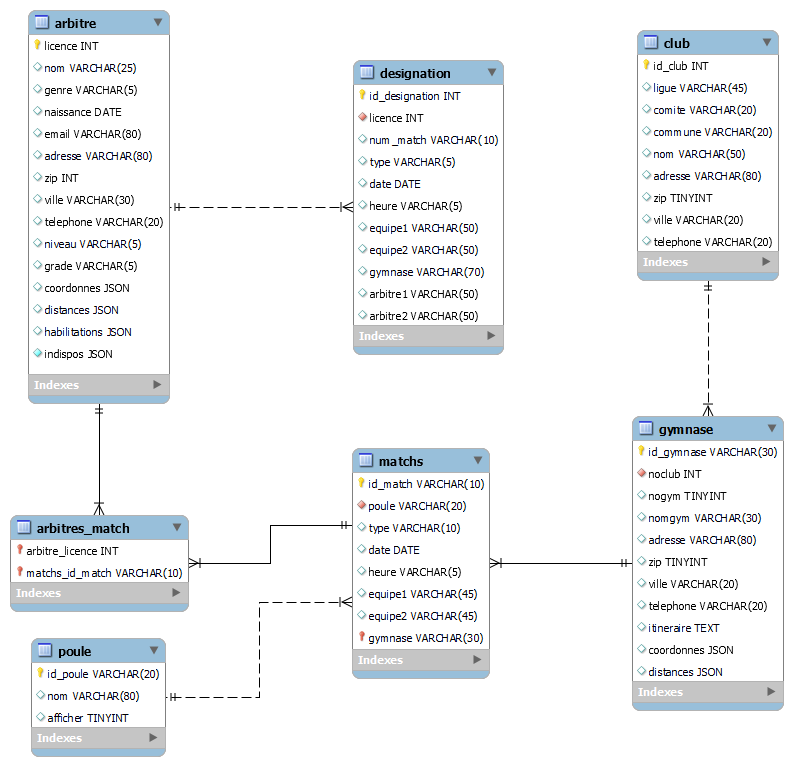
\includegraphics[width=\linewidth, height=15cm]{UML_DPP.png}
    \caption{Modèle de données UML effectué avec MySQL Workbench}
\end{figure}

\vspace{0.5cm}

Certaines données étaient disponibles au format csv (Excel), et d’autres demandaient à être récupérées sur l’intranet actuel de la fédération. Il m’a donc fallu extraire ces dernières via Web Scrapping pour ensuite les insérer dans ma base de données.